\section{Experiments}
\label{sec:experiments}

We apply the outlined methods to a variety of labelled networks. For reference, the inferred partitions for all of these are potted on Figure~\ref{fig:graphs-all}.

\begin{itemize}
	\item \textbf{Political books} \cite{polbooks} ($N=105, E=441, D=3$) -- network of Amazon political book sales, published close to the 2004 presidential election. Two books are connected if they were frequently co-purchased. Vertex features encode the political affiliation of the author (liberal, conservative, or neutral).
	\item \textbf{Primary school dynamic contacts} \cite{schools} ($N=238, E=5539, D=13$) -- network of face-to-face contacts amongst students and teachers at a primary school in Lyon, France. Vertex features include class membership (one of 10 values: 1A-5B), gender (male, female) and teacher status encoded as an 11th school-class. We choose to analyse just the second day of results.
	\item \textbf{Facebook egonet} \cite{fb-snap} ($N=747, E=30025, D=480$) -- an assortment of Facebook users' friends lists. Vertex features are fully anonymised and encode information about each user's education history, languages spoken, gender, home-town, birthday etc. We focus on the egonet with id 1912.
\end{itemize}
%
We first require metrics to assess model performance. We define the average
description length per entity (nodes and edges) $\bar{S}_e$ as a suitable metric to gauge the SBM fit:
%
\begin{equation}
	\bar{S}_e \coloneqq \frac{1}{(N+E) |\Tcal_b|} \sum_{t\in \Tcal_b} S \left( b^{(t)} \right).
	\label{eqn:mean-dl}
\end{equation}

Next, to assess the performance of the feature-to-block predictor, 
we randomly partition the vertex set $[N]$ such that a constant fraction $f$ forms our training set $\Gcal_0$ and the remainder form our test set $\Gcal_1$.
The $b$-chain is run using the whole network but we only use vertices $v \in \Gcal_0$ to train the $\theta$-chain. As $|\Gcal_0| \neq |\Gcal_1|$ in general, we use the average cross-entropy loss 
over each set to gauge fit,
%
\begin{equation}
	\bar{\Lcal}_\star \coloneqq \frac{1}{|\Tcal_\theta|} \sum_{t \in \Tcal_\theta} \Lcal_\star^{(t)},
	\quad \textrm{where} \quad
	\Lcal_\star^{(t)} \coloneqq \frac{1}{|\Gcal_\star|} \sum_{i \in \Gcal_\star}\sum_{j \in [B]} \hat{y}_{ij} \log \frac{1}{\phi_j \left(x_i; \theta^{(t)} \right)},
	\label{eqn:cross-entropy-loss}
\end{equation}
%
where $\star \in \{0, 1\}$ toggles between the training and test sets.
%
Nevertheless, the cross-entropy loss is a coarse measure of fit. We wish to define a new measure of fit specific to each detected block. Let us define
$
	\Bcal_\star(j) \coloneqq \{i \in \Gcal_\star : \hat{b}_i = j\}
$
where
$ 
	\hat{b}_i \coloneqq \argmax_j \hat{y}_{ij}.
$
Now $\Bcal_\star(j)$ is the set of vertices that have maximum a posteriori probability of belonging to block $j$. We now define the {\em block-accuracy} for block $j$ as in \ref{eqn:accuracy}. This effectively tests whether the feature-to-block and the graph-to-block predictions agree in their largest component.
%
\begin{equation}
	\eta_\star(j) \coloneqq \frac{1}{|\Bcal_\star (j)| \cdot 
	|\Tcal_\theta| } 
	\sum_{i \in \Bcal_\star (j)}  \sum_{t \in \Tcal_\theta}
	\one \left\{\hat{b}_i = \argmax_j \phi_j \left( x_i; \theta^{(t)} \right) \right\}.
	\label{eqn:accuracy}
\end{equation}

\begin{table}[!ht]
	\centering
	\caption{Results averaged over $n=10$ iterations (mean $\pm$ std. dev.).}
	\label{tab:results}
	\resizebox{\textwidth}{!}{%
		\begin{tabular}{c|ccc|c|cc|ccc}
			Dataset  & $B$ & $D$ & $D'$ & $\bar{S}_e$ & $\bar{\mathcal{L}}_0$ & $\bar{\mathcal{L}}_1$ & $c^*$ & $\bar{\mathcal{L}}_0'$ & $\bar{\mathcal{L}}_1'$  \\ \hline
			Polbooks & 3 & 3 & -- & $2.250 \pm 0.000$ & $0.563 \pm 0.042$ & $0.595 \pm 0.089$ & -- & -- & -- \\
			School & 10 & 13 & 10 & $1.894 \pm 0.004$ & $0.787 \pm 0.127$ & $0.885 \pm 0.129$ & $1.198 \pm 0.249$ & $0.793 \pm 0.132$ & $0.853 \pm 0.132$ \\
			FB egonet & 10  & 480 & 10 & $1.626 \pm 0.003$ & $1.326 \pm 0.043$ & $1.538 \pm 0.069$ & $0.94 \pm 0.019$ & $1.580 \pm 0.150$ & $1.605 \pm 0.106$
		\end{tabular}
	}
\end{table}

\begin{figure}[!ht]
	\centering
	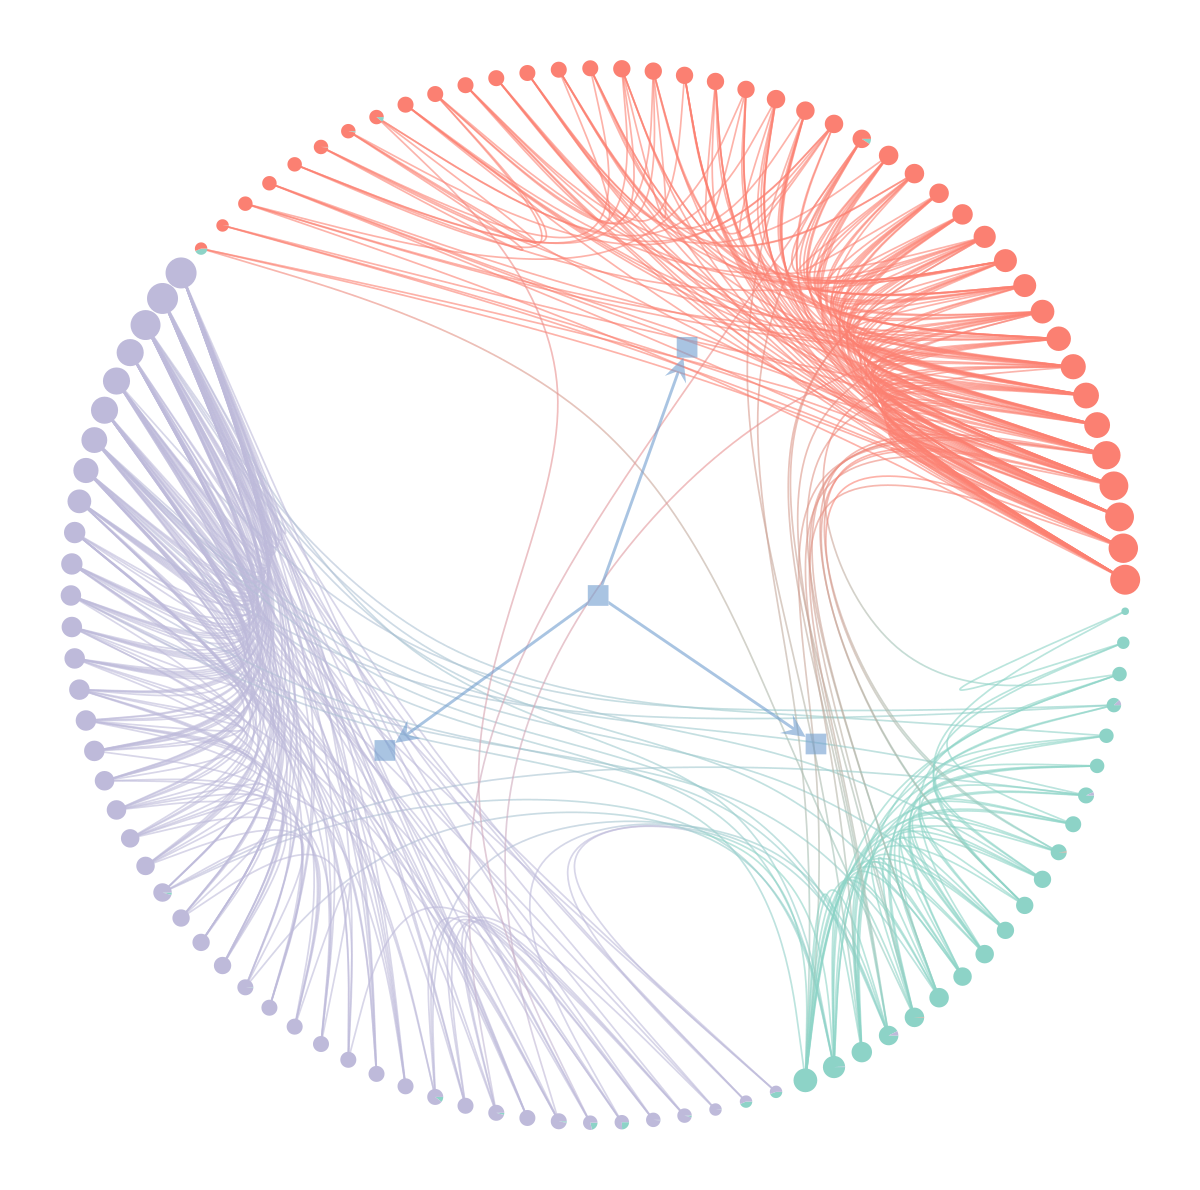
\includegraphics[width=0.28\linewidth]{img/polbooks-graph.png}
	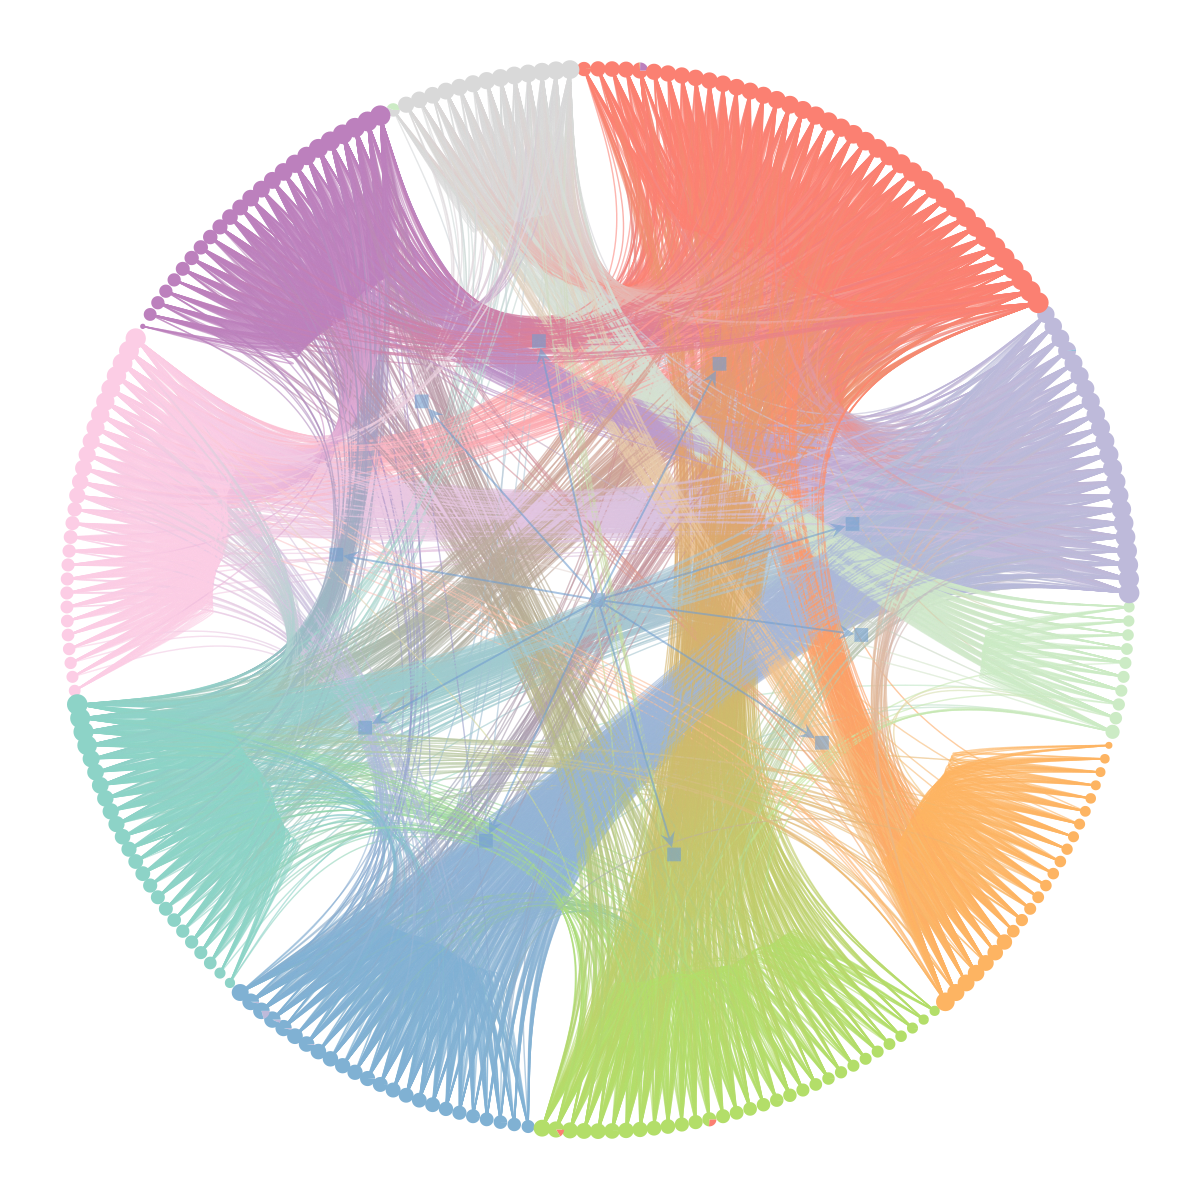
\includegraphics[width=0.28\linewidth]{img/school-graph.png}
	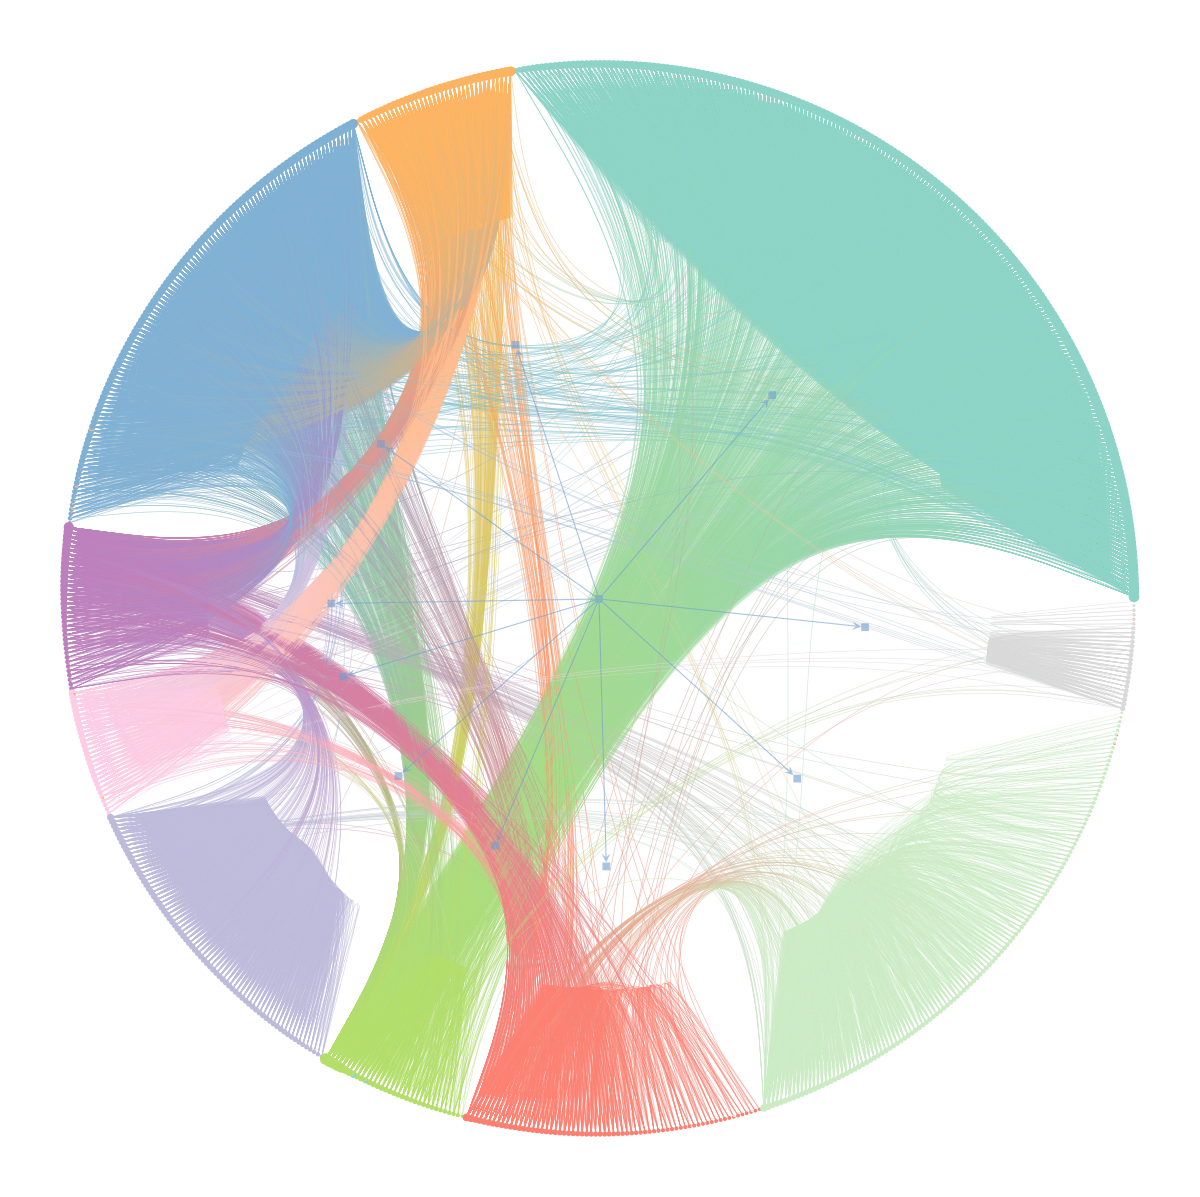
\includegraphics[width=0.28\linewidth]{img/fb-graph.png}
	\caption{Networks laid out and coloured according to inferred block memberships. Left to right: Polbooks, Krebs (2004); Primary School, Stehle et al (2011); Facebook Egonet, Leskovec and Mcauley (2012).}
	\label{fig:graphs-all}
\end{figure}

Table~\ref{tab:results} summarises the results for each experiment. 
We see that the dimensionality reduction procedure 
brings the training and test losses closer together. This implies that 
the features we keep are indeed correlated with the underlying graphical 
partition and that the approach generalises correctly. The test loss variance is higher than the training loss variance as the test set is smaller and so more susceptible to variability in its construction.
%
The average description length per entity,
$\bar{S}_e$, of the graph, 
has very small variance, suggesting that
the detected communities can be found reliably (to within an arbitrary 
relabelling of blocks).

\paragraph{\textbf{Political books.}}

We choose to partition the network into $B=3$ communities as we only have this many distinct values for political affiliation.
From Figure~\ref{fig:polbooks-null} we see that all 3 blocks have a distinct political affiliation as their largest positive component.  
Furthermore, the training and test losses from Table~\ref{tab:results}  
are very similar and both are low in magnitude. This is strong evidence 
that political affiliation is a very appropriate explanatory 
variable for the overall network structure.
%
However, from Figure~\ref{fig:polbooks-accuracy} we see that block 1 has low accuracy. 
This suggests that detected block 1 is not solely composed of ``neutral" books but also 
contains some ``liberal" and ``conservative" authors. Examining 
Figure~\ref{fig:polbooks-graph}, we see the majority of paths between blocks 2 and 3 go through block 1.
Block 1 is in effect a bridge between the ``conservative'' and ``liberal'' blocks so it is unsurprising that some of these leak into block 1.

\paragraph{\textbf{Primary school.}}

We choose the number of communities $B=10$, in line with the total number of 
school classes. Only the pupils' class memberships (1A-5B) survive
the dimensionality-reduction process (Figure~\ref{fig:school-null});
gender and teacher/student status have been discarded,
meaning these are poor predictors of overall macro-structure.
%
The vast majority of blocks are composed of a single class. 
However, some blocks have two comparably strong classes as their predictors (e.g. blocks 2 and 5). 
Conversely, some classes are found to extend over two 
detected blocks (class 2B spans blocks 8 and 9) but we do 
not have a feature which explains the division.
%
Figure~\ref{fig:school-accuracy} shows excellent accuracy for the majority of blocks. In fact the only blocks with low accuracy are those that have a school-class span two blocks such that we cannot reliably distinguish between the two. This is more pronounced when we apply hard classification rather than the soft cross-entropy loss. Perhaps there are unobserved features which explain this divide.

\paragraph{\textbf{Facebook egonet.}}

The retained features 
(Figure~\ref{fig:fb-null}) are those that best explain the high-level 
community structure. The majority of these are education related. 
Nevertheless, for $D'=10$ we only have good explanations for some of the detected blocks; several blocks in 
Figure~\ref{fig:fb-null} do not have high-magnitude components. This is further emphasised by the disparate accuracies in Figure~\ref{fig:fb-accuracy}.
%
For a high-dimensional feature-space, it is likely that a particular
feature may uniquely identify a small set of vertices; if these are all in the same block, then the classifier may overfit despite the penalty imposed by the prior. Indeed, we see in
Figure~\ref{fig:fb-null} that the feature birthday-5 has a very high weight as it relates to block 1 – but it is unlikely that birthdays determine graphical structure.

